%
% Demonstration of using statistical method to compute the value of π.
% Written in summer 2024.
%

\documentclass[tikz]{standalone}
\begin{document}
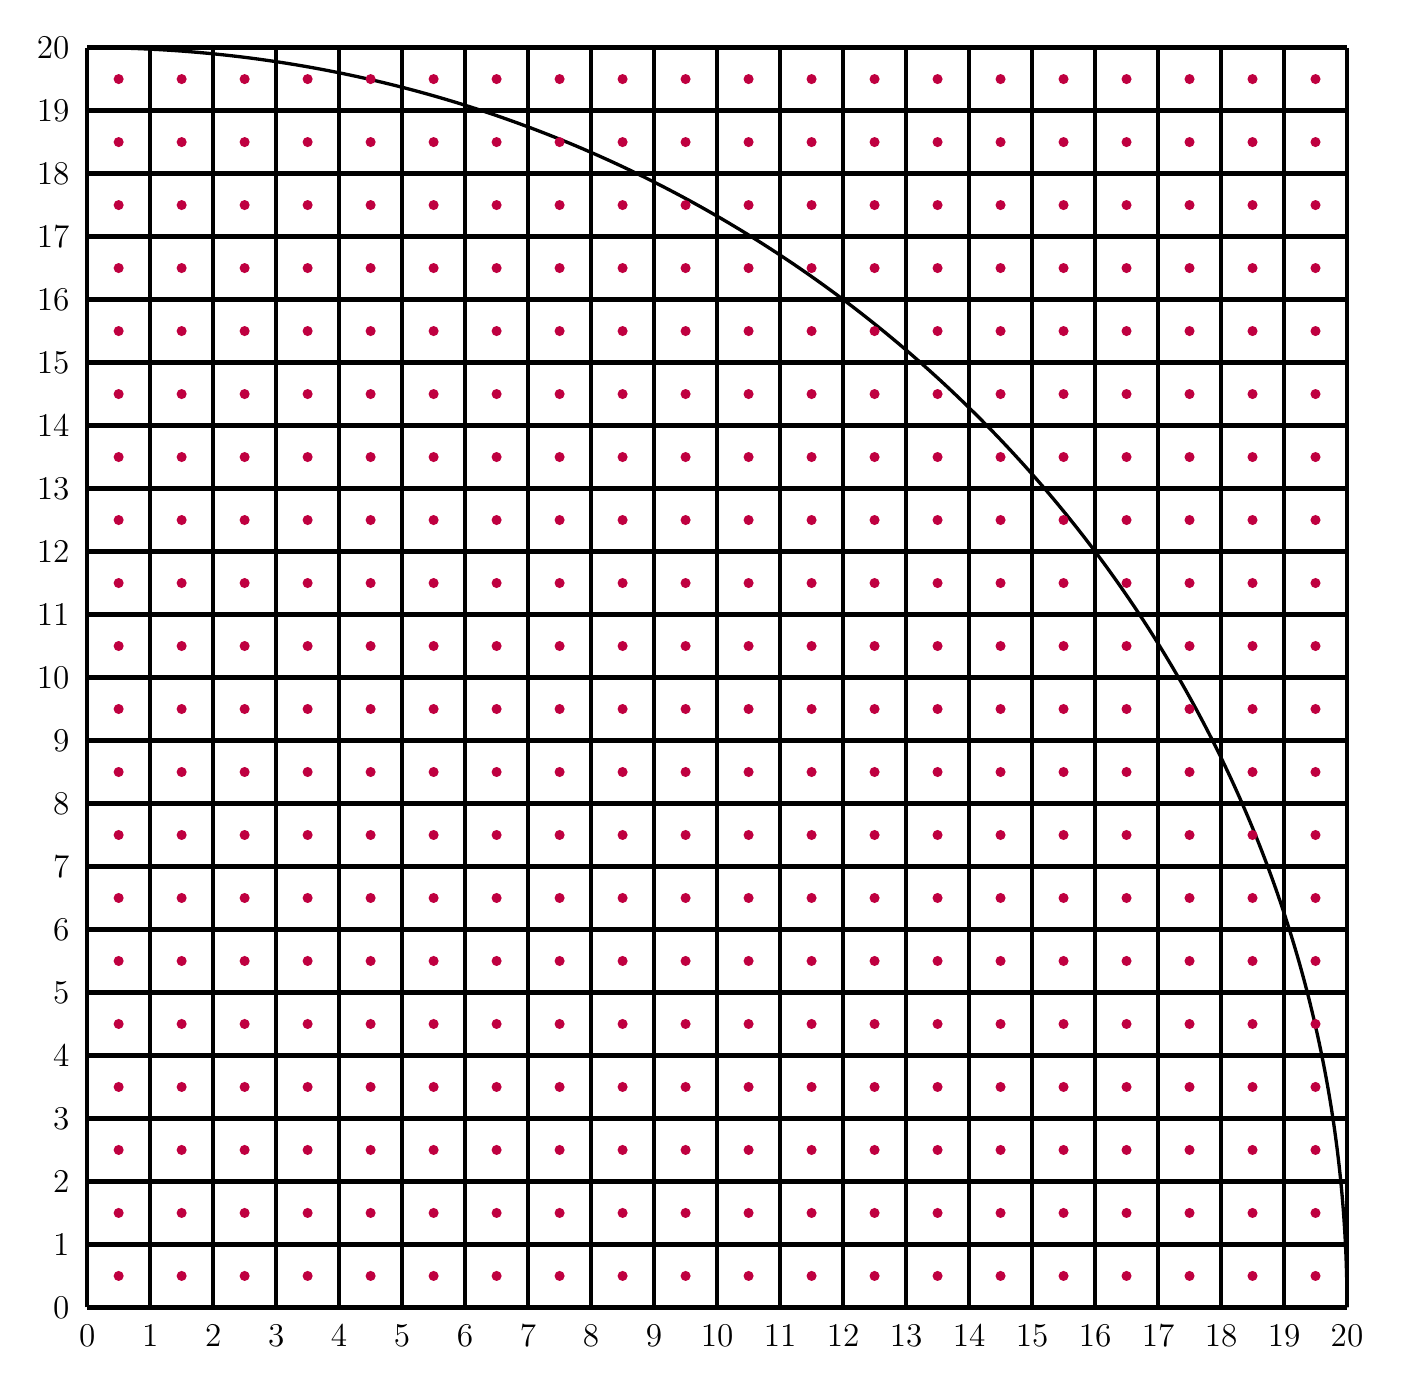
\begin{tikzpicture}[
  scale=0.8,
  every path/.append style={ultra thick},
  font=\large
  ]
  \draw (0,0) grid (20,20);
  \draw [very thick] (20,0) arc[start angle=0,end angle=90, x radius=20, y radius=20];
  \foreach \i in {0,1,...,20} {
    \node [anchor=north] at (\i,-0.1) {\i};
    \node [anchor=east] at (-0.1,\i) {\i};
  }

  \foreach \x in {1,...,20} {
    \foreach \y in {1,...,20} {
      \draw[fill=purple,draw=none](\x-0.5,\y-0.5)circle(0.08);
    }
  }
\end{tikzpicture}
\end{document}